% L14a (copy of L15a) preference weights with updated estimates. One time axis with three rows.
% Top: a path of the market state xi_t, red where the market is falling (xi_t > 0) and blue
% where it is rising (xi_t < 0). Middle: the estimates and the preference weights update
% every trading day (one dot per day). Bottom: the gamma basket the method holds, which changes only on a
% pick day: every 21 trading days, and on a market turn (orange line), the day xi_t is on
% the other side of zero from its value on the last pick day. A pick at a turn restarts the
% 21-day count (pick_days in week-15/L15a/src/Helper.jl). Basket 2 lasts 15 trading days (days 21 to 36):
% the first turn cuts it short.
%
% November 20, 2026: drawn in the style of the L13a schematics (schematic-style.tex).
% November 24, 2026: copied from week-15/L15a/figs (Fig-L15a-Gamma-Picks) for the closing question of L14a.
% The xi_t path is made up: 0.65 sin(2 pi (d - 35.5)/120), d = 0..132, 12/126 cm per day; the
% pick days 0, 21, 36 (turn), 57, 78, 96 (turn), 117 follow pick_days.
\documentclass[tikz,border=6pt]{standalone}
% Shared style for the L14a schematics (November 19, 2026), \input by each Fig-L14a-*.tex.
% Copied from week-13/L13a/figs/jumphmm-diagram.tex (the week-12 schematic style): same fonts,
% ink, accent colors, boxes, and arrows, plus a monospace font for tool names and order
% statuses. The notebook SVG carries a dark palette added by theme_svg.py; every color here
% must be mapped there.
\usepackage[no-math]{fontspec}
\IfFontExistsTF{Arial}{\setsansfont{Arial}}{\setsansfont{TeX Gyre Heros}}
\renewcommand{\familydefault}{\sfdefault}
\IfFontExistsTF{Menlo}{\setmonofont[Scale=0.92]{Menlo}}{}
\usepackage{amsmath,amssymb}
\usetikzlibrary{arrows.meta,calc,positioning,decorations.pathreplacing}

\definecolor{vnink}{HTML}{202124}
\definecolor{gdblue}{HTML}{0091FF}
\definecolor{gdred}{HTML}{E02020}
\definecolor{gdgray}{HTML}{6D7278}
\definecolor{saorange}{HTML}{F08C00}
\definecolor{boxfill}{HTML}{F1F3F4}
\definecolor{orangefill}{HTML}{FFE8C7}
\definecolor{bluefill}{HTML}{E5F3FF}
\definecolor{redfill}{HTML}{FDE8E8}
\definecolor{gridgray}{HTML}{E3E5E8}

\tikzset{
  every picture/.append style={x=1cm, y=1cm, font=\sffamily\small, text=vnink},
  % boxes and arrows, as in the L12a schematics
  flow/.style={draw=vnink, line width=0.9pt, -{Latex[length=2.4mm, width=1.7mm]}},
  feedback/.style={draw=saorange, line width=1.2pt, -{Latex[length=2.6mm, width=1.9mm]}, rounded corners=6pt},
  sumbox/.style={draw=vnink, fill=boxfill, line width=0.8pt, rounded corners=3pt, inner sep=5pt, align=center},
  note/.style={text=gdgray, font=\sffamily\footnotesize, align=center},
  state/.style={circle, draw=vnink, fill=white, line width=1.0pt, minimum size=1.1cm, inner sep=0pt, font=\sffamily\normalsize},
  % plots, as in the L10b profit diagrams
  axis/.style={draw=vnink, line width=0.8pt, -{Latex[length=2.6mm, width=1.8mm]}},
  spine/.style={draw=vnink, line width=0.8pt},
  curve/.style={draw=vnink, line width=1.6pt, line join=round, line cap=round},
  series/.style={draw=gdgray, line width=0.9pt, line join=round},
  drop/.style={draw=gdgray, line width=0.8pt, dash pattern=on 3pt off 2pt},
  pt/.style={circle, draw=vnink, fill=white, line width=1.0pt, inner sep=0pt, minimum size=2.0mm},
}


\begin{document}
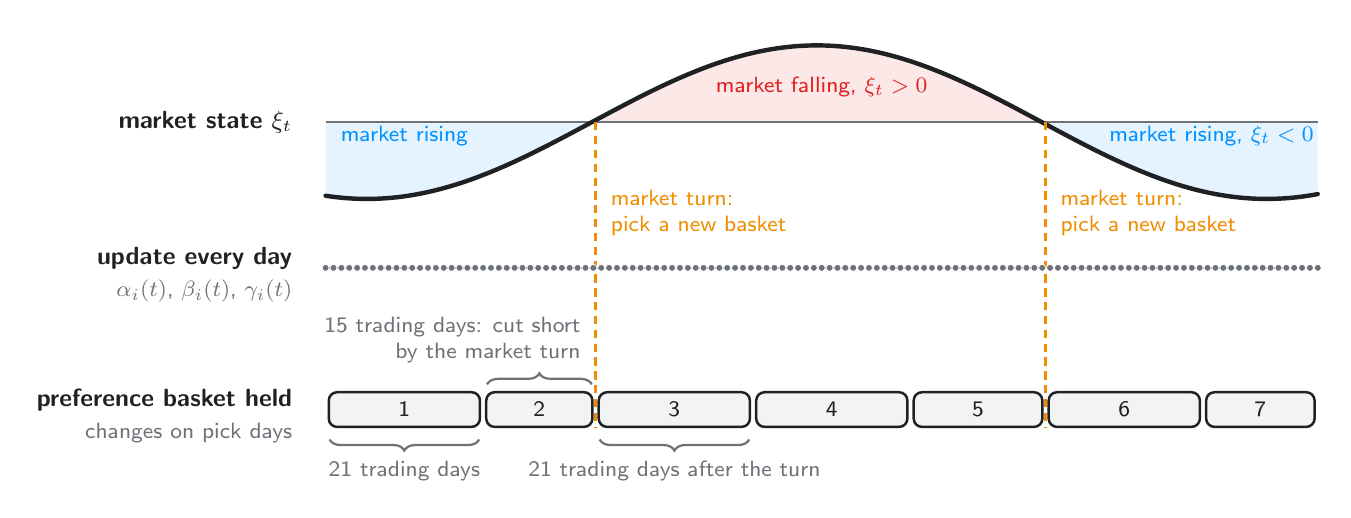
\begin{tikzpicture}[
  label/.style={font=\sffamily\small\bfseries, anchor=east, align=right},
  held/.style={draw=vnink, fill=boxfill, line width=0.9pt, rounded corners=3pt},
]
  % ---------------------------------------------------------------- the market state
  \begin{scope}[shift={(0, 4.2)}]
    \begin{scope}
      \clip (0, 0) rectangle (12.6, 1.2);
      \fill[redfill] (0, 0) -- plot[domain=0:12.6, samples=240] (\x, {1.5*0.65*sin(31.5*\x - 106.5)}) -- (12.6, 0) -- cycle;
    \end{scope}
    \begin{scope}
      \clip (0, -1.2) rectangle (12.6, 0);
      \fill[bluefill] (0, 0) -- plot[domain=0:12.6, samples=240] (\x, {1.5*0.65*sin(31.5*\x - 106.5)}) -- (12.6, 0) -- cycle;
    \end{scope}
    \draw[spine, draw=gdgray] (0, 0) -- (12.6, 0);
    \draw[curve] plot[domain=0:12.6, samples=240] (\x, {1.5*0.65*sin(31.5*\x - 106.5)});
    \node[font=\sffamily\footnotesize, text=gdred] at (6.3, 0.45) {market falling, $\xi_{t}>0$};
    \node[font=\sffamily\footnotesize, text=gdblue] at (1.0, -0.17) {market rising};
    \node[font=\sffamily\footnotesize, text=gdblue] at (11.25, -0.17) {market rising, $\xi_{t}<0$};
    \node[label] at (-0.3, 0) {market state $\xi_{t}$};
    % the turns
    \draw[drop, draw=saorange] (3.4286, 0) -- (3.4286, -3.87);
    \draw[drop, draw=saorange] (9.1429, 0) -- (9.1429, -3.87);
    \node[note, anchor=west, text=saorange, align=left] at (3.5, -1.15) {market turn:\\pick a new basket};
    \node[note, anchor=west, text=saorange, align=left] at (9.21, -1.15) {market turn:\\pick a new basket};
  \end{scope}

  % ---------------------------------------------------------------- the daily update
  \begin{scope}[shift={(0, 2.35)}]
    \draw[draw=gdgray, line width=0.6pt] (0, 0) -- (12.6, 0);
    \foreach \d in {0, ..., 126} {
      \filldraw[fill=gdgray, draw=white, line width=0.3pt] (0.1*\d, 0) circle (0.045);
    }
    \node[label] at (-0.3, 0.12) {update every day};
    \node[note, anchor=east] at (-0.3, -0.3) {$\alpha_{i}(t)$, $\beta_{i}(t)$, $\gamma_{i}(t)$};
  \end{scope}

  % ---------------------------------------------------------------- the basket held
  \begin{scope}[shift={(0, 0.55)}]
    \foreach \a/\b/\n in {0.0/2.0/1, 2.0/3.4286/2, 3.4286/5.4286/3, 5.4286/7.4286/4, 7.4286/9.1429/5, 9.1429/11.1429/6, 11.1429/12.6/7} {
      \draw[held] (\a + 0.04, -0.22) rectangle (\b - 0.04, 0.22);
      \node[font=\sffamily\footnotesize] at ({(\a + \b)/2}, 0) {\n};
    }
    \node[label] at (-0.3, 0.12) {preference basket held};
    \node[note, anchor=east] at (-0.3, -0.3) {changes on pick days};
    \draw[decorate, decoration={brace, amplitude=4pt, mirror}, draw=gdgray, line width=0.8pt] (0.05, -0.38) -- (1.95, -0.38);
    \node[note, anchor=north] at (1.0, -0.53) {21 trading days};
    \draw[decorate, decoration={brace, amplitude=4pt, mirror}, draw=gdgray, line width=0.8pt] (3.48, -0.38) -- (5.38, -0.38);
    \node[note, anchor=north] at (4.43, -0.53) {21 trading days after the turn};
    \draw[decorate, decoration={brace, amplitude=4pt}, draw=gdgray, line width=0.8pt] (2.05, 0.32) -- (3.38, 0.32);
    \node[note, anchor=south east, align=right] at (3.36, 0.47) {15 trading days: cut short\\by the market turn};
  \end{scope}
\end{tikzpicture}
\end{document}
